\documentclass[border=10pt]{standalone}
\usepackage{pgfplots}
\pgfplotsset{compat=1.18}
\begin{document}
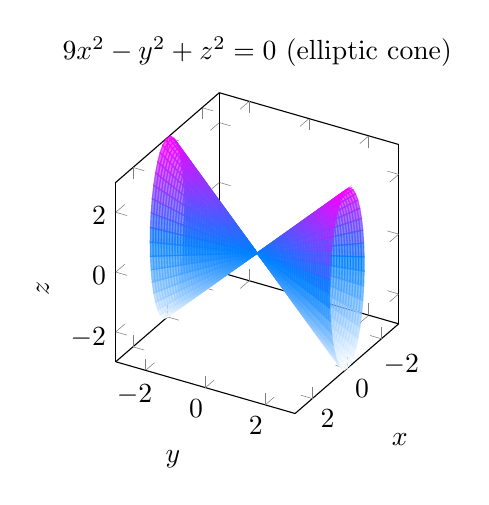
\begin{tikzpicture}
\begin{axis}[
    view={120}{30},
    xlabel=$x$, ylabel=$y$, zlabel=$z$,
    xmin=-3, xmax=3,
    ymin=-3, ymax=3,
    zmin=-3, zmax=3,
    samples=40, samples y=40,
    colormap/cool,
    title={$9x^2-y^2+z^2=0$ (elliptic cone)},
    axis equal image,
]
\addplot3[surf, domain=0:360, y domain=0:3, shader=flat, opacity=0.7] ({y/3*cos(x)}, {y}, {y*sin(x)});
\addplot3[surf, domain=0:360, y domain=0:3, shader=flat, opacity=0.7] ({y/3*cos(x)}, {-y}, {y*sin(x)});
\end{axis}
\end{tikzpicture}
\end{document}